\documentclass{article}

% If you're new to LaTeX, here's some short tutorials:
% https://www.overleaf.com/learn/latex/Learn_LaTeX_in_30_minutes
% https://en.wikibooks.org/wiki/LaTeX/Basics

% Formatting
\usepackage[utf8]{inputenc}
\usepackage[margin=1in]{geometry}
\usepackage[titletoc,title]{appendix}

% Math
% https://www.overleaf.com/learn/latex/Mathematical_expressions
% https://en.wikibooks.org/wiki/LaTeX/Mathematics
\usepackage{amsmath,amsfonts,amssymb,mathtools}

% Images
% https://www.overleaf.com/learn/latex/Inserting_Images
% https://en.wikibooks.org/wiki/LaTeX/Floats,_Figures_and_Captions
\usepackage{graphicx,float}

% Tables
% https://www.overleaf.com/learn/latex/Tables
% https://en.wikibooks.org/wiki/LaTeX/Tables

% Algorithms
% https://www.overleaf.com/learn/latex/algorithms
% https://en.wikibooks.org/wiki/LaTeX/Algorithms
\usepackage[ruled,vlined]{algorithm2e}
\usepackage{algorithmic}

% Code syntax highlighting
% https://www.overleaf.com/learn/latex/Code_Highlighting_with_minted
\usepackage{listings}
%\usepackage{minted}
%\usemintedstyle{borland}

\usepackage{hyperref}
\usepackage{subcaption}
\usepackage{bm}

% References
% https://www.overleaf.com/learn/latex/Bibliography_management_in_LaTeX
% https://en.wikibooks.org/wiki/LaTeX/Bibliography_Management
%\usepackage{biblatex}
%\addbibresource{references.bib}

% Title content
\title{AMATH 582 Homework One: Submarine Hunt}
\author{Daniel W. Crews}
\date{January 27, 2021}

\begin{document}

\maketitle

% Abstract
\begin{abstract}
    Signal processing is used ubiquitously in science and engineering. This simple numerical experiment explores an important aspect of signal analysis, namely statistical averaging of a spectral time series to eliminate noise and thereby identify center frequencies. Here the time series consists of a spatial wavefield which is denoised via Gaussian filtering about the identified frequency to determine a trajectory. While the technique explored in this report is quite elementary compared to more sophisticated signal processing approaches, it conveys the essential elements of, for example, a radar or sonar tracking system. %In this case such a trajectory is determined from a noisy waveform in a time series of three spatial dimensions. 
\end{abstract}

% Introduction and Overview
\section{Introduction}
The premise of this analysis is to track the location of a submarine given a noisy spatial wavefield constructed somehow through acoustic measurements. Given that noise is random, it may be supposed (for instance via the central limit theorem) that it is normally distributed with zero mean and some variance. Therefore it is expected to vanish upon time average. As the submarine is moving, its location also smears over time average. Yet the submarine's spatial frequency is an analytic signature and remains upon time average, provided the average is over an interval small enough compared to the change in the submarine's shape or sound. This analysis assumes the target's signature to not change with time in the frequency domain.

This report describes an algorithm used to denoise the signal via a statistical method and to identify the submarine's trajectory. It begins with a brief theoretical overview of the methods used, and proceeds to a discussion of the details of the code used to implement the methods. There is then a discussion of results identifying the three-dimensional trajectory, along with a suggested search area for a submarine-tracking aircraft and the likely frequency of the submarine. The report is kept brief without sacrificing clarity.

%  Theoretical Background
\section{Theoretical Background}
\subsection{Spectral analysis, discrete Fourier series, and the FFT}
The Fourier series is an eigenfunction expansion of an integrable function $f(x)$ (or formally, satisfying the Dirichlet conditions) on a finite interval $x\in D$ of length $|D| = L$ into the series
\begin{equation}
    f(x) = \sum_{n=-\infty}^\infty c_ne^{ik_nx}, \quad\quad k_n = \frac{2\pi}{L}n
    \label{fseries}
\end{equation}
where the wavenumbers $k_n$ are integer multiples of the fundamental domain harmonic $k_1 = \frac{2\pi}{L}$ and the coefficients $c_n$ are given by the usual Fourier integrals \cite{lanczos2}. Given functional values $f_n$ on equally-spaced points $\{x_n\}|_{n=0}^{N-1}$, the ``discrete Fourier transform'' is a quadrature approximation of the Fourier integral,
\begin{equation}
  \hat{f}_m = \sum_{n=0}^{N-1}f_ne^{-ik_mx_n},\quad\quad f_n = \frac{1}{N}\sum_{m=0}^{N-1}\hat{f}_me^{ik_mx_n}\label{disc}
\end{equation}
The requirement that the points be equally spaced is quite important. The reason is revealed by supposing the functional values $f_n$ to interpolate a piecewise constant function $\widetilde{f}(x)$ on the interval $D$, with each subinterval centered about each point $x_n$ and with width $\Delta x_n$. The Fourier integral of $\widetilde{f}(x)$ yields coefficients
\begin{equation}
  c_n = \frac{1}{L}\sum_{m=0}^{N-1}\frac{\Delta x_m}{2} \text{sinc}\Big(\frac{\Delta x_m}{2}k_n\Big)e^{-ik_nx_m}f_m\label{sinc}
\end{equation}
where the cardinal sine function $\text{sinc}(x) = \sin(x)/x$ is the spectral signature of the interval $\Delta x_m$. If the interval widths $\Delta x_m$ are equal, then the sinc function factors out of the series and the expression may be inverted. Inversion takes place on account of the discrete orthogonality property of the circle functions,
\begin{equation}
  \frac{\pi}{n}\sum_{\alpha=-n}^n\sin\Big(k\frac{\pi}{n}\alpha\Big)\sin\Big(m\frac{\pi}{n}\alpha\Big) = \delta_{nm},
\end{equation}
a property noted by at least 1759 by Lagrange, though he did not take the last steps to the full Fourier series as the appropriate limiting notions were not fully understood in those times \cite{lanczos}.

This procedure results in a discrete transform pair provided that the intervals are equally spaced. If the spacings are not equal, each interval's spectral signature is tangled up with its phase information and such a simple discrete inversion is not possible. In such a case, one must interpolate onto equally-spaced intervals. Note that Eqn. \ref{sinc} is the zeroth-order interpolant transform. The spectral signature of \textit{e.g.} higher-order Legendre polynomial interpolants are the spherical Bessel functions, of which $\text{sinc}$ is the first member.

The fast Fourier transform (FFT) is an algorithm to compute the discrete Fourier transform of Eqn. \ref{disc} on a set of $N$ equally-spaced points in $\mathcal{O}(N\log(N))$ operations. If the set consists of $N = 2^M$ points then even more efficient transformation is possible. In Cartesian coordinates the multidimensional discrete Fourier transform is obtained by that of each dimension independently, as the kernel $e^{i\bm{k}\cdot\bm{x}}$ factorizes the Fourier integral into one-dimensional transforms\footnote{Note that for more specialized geometries such as polar coordinates one may define discrete versions of the relevant Fourier transforms, e.g. the Hankel transform and its discrete counterpart. It is intriguing to observe that in polar coordinates the Fourier series arises even for infinite domains as the angular direction is naturally periodic.}. In this analysis the three-dimensional FFT is computed using Numpy's $\text{np.fft.fftn()}$ routine, and inverse transform via $\text{np.fft.ifftn()}$.

\subsection{Separation of mean and fluctuations}\label{mean_sect}
A goal of science and engineering is to separate the dynamics of a mean value from that of its fluctuations. The idea is that an interpretable signal $X$ consists of an orderly mean part $\langle X\rangle$ which follows some understandable rule of evolution, and a fluctuating part $\delta X$ whose precise nature is unknown (or even unknowable, if the intrinsic probability suggested by quantum mechanics is indeed true) \cite{vankampen}. The variable $X$ is decomposed by
\begin{equation}
  X = \langle X\rangle + \delta X.\label{avg}
\end{equation}
It is important to note that the fluctuations $\delta X$ may influence the observable evolution $\langle X\rangle$. Yet it is often the case that fluctuations are entirely independent of the mean dynamics. For instance, acoustic fluctuations in the Puget Sound due to wind and distant whale song do not change the sound of a submarine there. In such a case the goal is to eliminate the noise, and by the very definition of the splitting in Eqn. \ref{avg}, averaging of the signal $X$ over an appropriate window of samples will substantially reduce the presence of $\delta X$ \cite{kutz}. By this method all coherent sources will be determined and the fluctuations suppressed.

\subsection{The exponential filter}
The averaging procedure obscures information within the sampling window. Yet once the coherent source is identified through averaging, one may then filter the original data within the window to denoise and isolate the source. A common filter utilized is the exponential one in $d$-dimensions,
\begin{equation}
  \mathcal{F}(\bm{k};\bm{k}_0) = \exp\Big(-\tau\sum_{i=0}^{d-1}(k_i - k_{0,i})^{\sigma}\Big)\label{filter}
\end{equation}
where $\bm{k}_0$ is the center (vector) frequency, $\tau$ is a scaling (bandwidth) parameter, and $\sigma$ an even parameter giving the filter strength. The Gaussian filter is utilized in this analysis, corresponding to $\tau = 0.5$ and $\sigma = 2$.

% Algorithm Implementation and Development
\section{Analysis and discussion}
The data provided for analysis is supposed to be a spatial waveform determined through acoustic measurements, and consists of complex amplitudes on an evenly-spaced $N^3 = 64^3$ Cartesian grid discretizing a domain of $L = 10$ spatial units, with 49 time measurements taken in half-hour intervals. As an objective is to identify the frequency of the submarine, the averaging described in Section \ref{mean_sect} is applied to the Fourier transform of the given data. By determining the submarine frequency, inversion of the filtered spectrum is used to detect the submarine's location for each of the 49 recorded half-hour steps.

\subsection{Algorithm schematic}
The following list gives a simple overview of the steps used for trajectory identification, along with the associated Numpy functions for implementation of the FFT:
\begin{enumerate}
\item \textbf{Initialize:} The data is read in ($n=64$), and the spatial and spectral grids initialized;
  \begin{itemize}
  \item The evenly-spaced spatial grid via \texttt{x=\text{np.linspace(-L, L, num=n+1)}}, and the corresponding wavenumbers (scaled to angular frequency by $\times 2\pi$, as the Numpy FFT returns frequencies in Hertz) using \texttt{np.fft.fftfreq} (see App. \text{functions} for details).
  \end{itemize}
\item \textbf{Transform, time average:} The spectrum is found via FFT for each timestep. It is then averaged over a window of seven time samples, or three and a half hours (chosen as the square-root of 49; it was found to work in this case).
\item \textbf{Find center frequency:} The center frequency in each averaged time window is found by computing the mean wavenumber of all points greater than a $70\%$ detection threshold.
\item \textbf{Spectral filter:} For each time $t$, the spectrum is denoised by applying a Gaussian filter (Eqn. \ref{filter} with $\tau = 0.5$ and $\sigma=2$) about the center frequency $k_{0}$ determined in Step 3 for that window $t\in|T_i|$.
\item \textbf{Inverse transform and trajectory:} The denoised spectrum is transformed back to the spatial domain, and the mean location of all points above an $80\%$ detection threshold is considered to be the submarine's location.
\end{enumerate}
Note that the detection threshold is set by the operator, according to the degree of various signals persisting after time averaging. The $70\%$ and $80\%$ detection thresholds were seen to work quite well. For further information, Appendix \ref{functions} details some Python functions while Appendix \ref{implementation} contains code implementation. Github repository for this work is available \href{https://github.com/crewsdw/amath582}{here}.

\subsection{Analysis results}
Initialization according to Step 1 in the schematic allowed visualization of the dataset via an isosurface, as in Fig. \ref{iso}. The signal is clearly visible to the eye in this plot, and was confirmed as a real object by time-averaging of the frequency spectrum over a set of seven time measurements. Time-averaging of the frequency is critical, as the object is moving so that its average position is not constant. However, the object's spectral signature is unchanged as it did not change shape (or did not change acoustic signature, as the nature of the data provided is obscure). Table \ref{frequencies} shows centers found by time averaging.

\begin{figure}[ht]
  \centering
  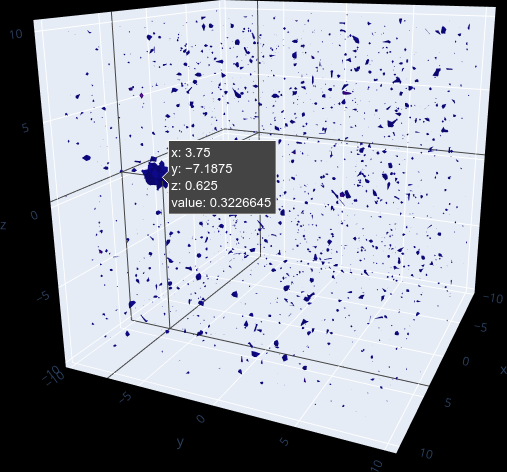
\includegraphics[width=0.5\textwidth]{pics/iso}
  \caption{Isosurface at $50\%$ maximum of acoustic data $|\psi(x,t=0)|/|\psi|_\infty$, revealing a noisy background field and an apparent signal with coordinates highlighted. Upon time-averaging in the frequency domain, the signal was confirmed to be coherent, i.e. have non-zero mean.}\label{iso}
\end{figure}

\begin{table}[b]
  \centering
  \begin{tabular}{|l|l|l|l|l|l|l|l|l|}
    \hline
    Time {[}hr{]}   & 0-3.5 & 3.5-7.0 & 7.0-10.5 & 10.5-14.0 & 14.0-17.5 & 17.5-21.0 & 21.0-24.5 & All-time average \\ \hline
    $\langle k_x\rangle_T$ {[}1/L{]} & 0.814 & 0.661   & 0.784    & 0.760     & 0.810     & 0.728     & 0.802     & 0.766            \\ \hline
    $\langle k_y\rangle_T$ {[}1/L{]} & 0.271 & 0.292   & 0.331    & 0.240     & 0.341     & 0.267     & 0.271     & 0.288            \\ \hline
    $\langle k_z\rangle_T$ {[}1/L{]} & -1.00 & -1.03   & -1.09    & -1.06     & -1.13     & -1.07     & -1.1125   & -1.07            \\ \hline
  \end{tabular}
  \caption{Observed center frequencies of data following spectral averaging over time intervals of $3.5$ hours, with seven samples per interval, then used as the filter frequencies $k_0$ in the Gaussian filter. The arbitrary spatial unit is given as $L$, not to be confused with domain length. The all-time average is given as well.}\label{frequencies}
\end{table}

Note that in Table \ref{frequencies} negative wavenumbers are used as the given spatial data is complex, meaning that the reality condition is not satisfied, instead $\hat{f}(-k) = \hat{f}^*(k)$ in this dataset. The absolute value is reported as ``the frequency'' of the submarine, however. This identifies the submarine's spectral signature as $\bm{k} \approx \{0.766 \pm 0.05, 0.288 \pm 0.03, 1.07 \pm 0.04 \}$ {[}1/L{]} by mean and standard deviation of the window averages of Table \ref{frequencies}, where L is an arbitrary space unit corresponding to that of the provided data, \textit{not} the domain length. The width of the space or frequency ``submarine Gaussian'' was not measured for ease of analysis.

Having computed the center frequencies, the spectrum was filtered and the trajectory determined according to the schematic Steps 4 and 5. The resulting 3D trajectory and top-down position given in Figs. \ref{traj:3d}, \ref{traj:2d} respectively. This suggests the submarine is currently located around $\bm{x}\sim(-5, 6.5)$ in $(x,y)$.

\begin{figure}[hb]
  \centering
  \begin{subfigure}{0.42\textwidth}
    \centering
    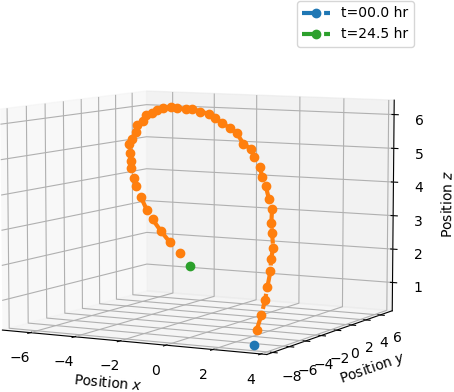
\includegraphics[width=0.99\linewidth]{pics/3d_traj}
    \caption{Three-dimensional trajectory of submarine, showing a rise and dive maneuver.}\label{traj:3d}
  \end{subfigure}
  \begin{subfigure}{0.42\textwidth}
    \centering
    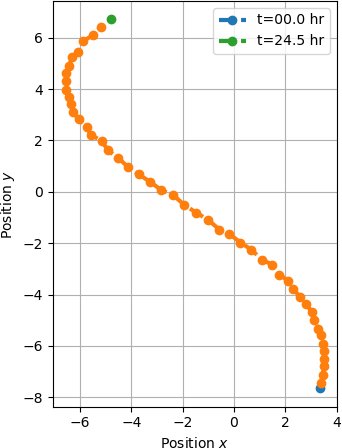
\includegraphics[width=0.68\linewidth]{pics/2d_traj}
    \caption{Top-down view of predicted trajectory. Ideal search area for submarine-tracking aircraft is around $\bm{x} \sim (-5, 6.5)$ and continuing north-east.}\label{traj:2d}
  \end{subfigure}
\end{figure}

% Summary and Conclusions
\section{Summary and Conclusions}
This numerical experiment combined Fourier spectral methods with statistical methods to analyze what is effectively sonar data by an elementary technique. Noise was eliminated by averaging of the frequency spectrum of a moving target, when averaging of the spatial position would be smeared away by motion. The trajectory was determined satisfactorily and the frequency signature of the object determined for future reference and classification. Finally, Python was used for implementation of this exercise, though Matlab may be used in the future if the required analysis is simpler that way.

% References
\bibliographystyle{unsrt}
\bibliography{references}

% Appendices
\begin{appendices}

% MATLAB Functions
\section{Python Functions}\label{functions}
The following list compiles important Python functions used in implementation:
\begin{itemize}
    \item \texttt{np.linspace(x1,x2,num=n)} returns a row vector of \texttt{n} evenly spaced points between \texttt{x1} and \texttt{x2}. 
    \item \texttt{np.meshgrid(x,y)} returns 2-D grid coordinates based on \texttt{x} and \texttt{y}, with 3-D available too.
    \item \texttt{np.fft.fftn(x)} computes n-dimensional Fourier transform of gridded data while \texttt{np.fft.ifftn(x)} does the inverse transform and \texttt{np.fft.fftfreq(n, d=dx)} computes the frequencies for a dataset of \texttt{n} points and sample spacing \texttt{dx} \textit{in Hz}.
    \item \texttt{np.where(X > a)} determines a Boolean indexing array wherever the array \texttt{X} is greater than value \texttt{a}. Any Boolean statement may be put into the input. This is a quite useful function.
\end{itemize}

% MATLAB Codes
\section{Python Implementation}\label{implementation}

\lstinputlisting{hw1.py}

% \begin{listing}[h]
% \inputminted{matlab}{example.m}
% \caption{Example code from external file.}
% \label{listing:examplecode}
% \end{listing}

\end{appendices}

\end{document}